\section{Visitor}

The visitor design pattern is a way of separating an algorithm from an object structure on which it operates. A practical result of this separation is the ability to add new operations to existent object structures without modifying the structures. It is one way to follow the open/closed principle. In essence, the visitor allows adding new virtual functions to a family of classes, without modifying the classes. Instead, a visitor class is created that implements all of the appropriate specializations of the virtual function. The visitor takes the instance reference as input and implements the goal through double dispatch.
% Description of the design pattern

\subsection*{Example}

Figure~\ref{fig:Visitor} presents the UML diagram of visitor design pattern of project \textit{Follow}. In this instance, the client for visitor design pattern is the program. \texttt{ArenaObjectVisitor} is playing the role of visitor design pattern that including \texttt{ArenaObjectVisitorAdapter} and  \texttt{RobotScanner}.

\begin{figure}[htb]
    \centering
    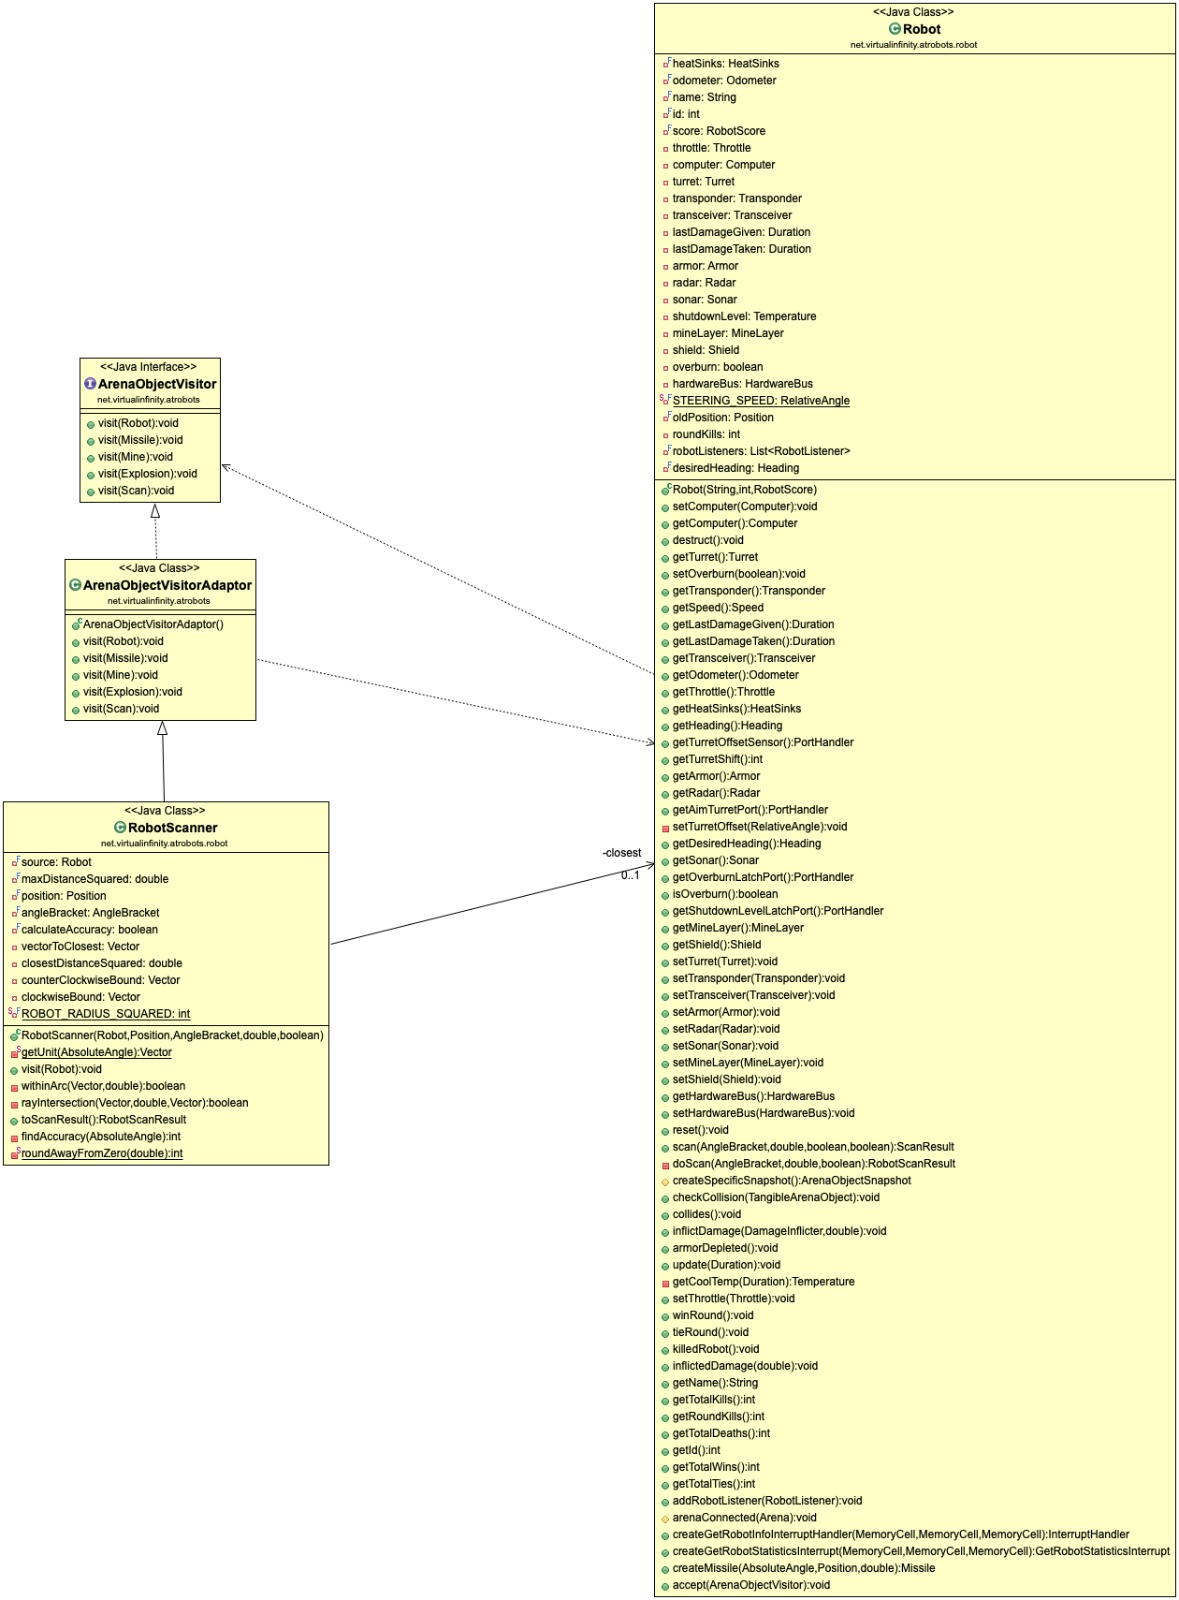
\includegraphics[width=\columnwidth]{images/Visitor.jpeg}
    \caption{Visitor design pattern in the project \textit{Follow}}
    \label{fig:Visitor}
\end{figure}
\FloatBarrier

% Description of the roles of the class in the design pattern

%---------------------------------------------------------------------------%
Figure~\ref{fig:Robot} is part of the class \texttt{Robot}'s code. In this instance \texttt{Robot} is playing the role of concrete elements. \\

\begin{figure}[htb]
\centering
\lstset{language=Java, basicstyle=\scriptsize, stepnumber=1, showspaces=false, showstringspaces=false,breaklines=true}
\begin{lstlisting}
public class Robot extends TangibleArenaObject implements Resettable, HasHeading, Destructable, HasOverburner, MissileFactory, ArmorDepletionListener, ScanSource, DamageInflicter {
    private final HeatSinks heatSinks = new HeatSinks();
    private final Odometer odometer = new Odometer();
    private final String name;
    private final int id;
    private final RobotScore score;
    private Throttle throttle;
    private Computer computer;
    private Turret turret;
    private Transponder transponder;
    private Transceiver transceiver;
    private Duration lastDamageGiven = Duration.fromCycles(0);
    private Duration lastDamageTaken = Duration.fromCycles(0);
   
    private Temperature shutdownLevel;
    private MineLayer mineLayer;
    private Shield shield;
    private boolean overburn;
    private HardwareBus hardwareBus;
    private static final RelativeAngle STEERING_SPEED = RelativeAngle.fromBygrees(8);
    private final Position oldPosition = new Position();
    private int roundKills;
    private final List<RobotListener> robotListeners = new ArrayList<RobotListener>();
    private final Heading desiredHeading = new Heading(heading.getAngle()); 
    
    {
        position.setOdometer(odometer);
    }

    public Robot(String name, int id, RobotScore score) {
        this.name = name;
        this.id = id;
        this.score = score;
        this.roundKills = 0;
    }

    public void setComputer(Computer computer) {
        this.computer = computer;
        computer.setId(getId());
        computer.setName(getName());
    }//other method


\end{lstlisting}
\caption{[Visitor] Robot.java}
\label{fig:Robot}
\end{figure}
\FloatBarrier

%---------------------------------------------------------------------------%
%---------------------------------------------------------------------------%



%---------------------------------------------------------------------------%
%---------------------------------------------------------------------------%
Figure~\ref{fig:RobotScanner} is part of the class \texttt{RobotScanner}'s code. In this instance \texttt{RobotScanner} is playing the role of concrete for visitor design pattern. 

\begin{figure}[htb]
\centering
\lstset{language=Java, basicstyle=\scriptsize, stepnumber=1, showspaces=false, showstringspaces=false,breaklines=true}
\begin{lstlisting}
public class RobotScanner extends ArenaObjectVisitorAdaptor {
    private final Robot source;
    private final double maxDistanceSquared;
    private final Position position;
    private final AngleBracket angleBracket;
    private final boolean calculateAccuracy;

    private Vector vectorToClosest = null;
    private double closestDistanceSquared;
    private Robot closest = null;
    private Vector counterClockwiseBound;
    private Vector clockwiseBound;
    private static final int ROBOT_RADIUS_SQUARED = 16;

    public RobotScanner(Robot source, Position position, AngleBracket angleBracket, double maxDistance, boolean calculateAccuracy) {
        this.source = source;
        this.position = position;
        this.angleBracket = angleBracket;
        this.calculateAccuracy = calculateAccuracy;
        this.counterClockwiseBound = getUnit(angleBracket.getCounterClockwiseBound());
        this.clockwiseBound = getUnit(angleBracket.getClockwiseBound());
        this.maxDistanceSquared = maxDistance * maxDistance;
        this.closestDistanceSquared = maxDistanceSquared;
    }

    private static Vector getUnit(AbsoluteAngle absoluteAngle) {
        if (absoluteAngle == null) {
            return null;
        }
        return absoluteAngle.toUnitVector();
    }

    public void visit(Robot arenaObject) {
        if (arenaObject == source) {
            return;
        }
        final Vector position = arenaObject.getPosition().getVectorTo(this.position);
        final double distanceSquared = position.getMagnitudeSquared();
        if (distanceSquared < closestDistanceSquared && withinArc(position, distanceSquared)) {
            closest = arenaObject;
            closestDistanceSquared = distanceSquared;
            vectorToClosest = position;
        }
    }

    private boolean withinArc(Vector position, double distanceSquared) {
        return angleBracket.contains(position.getAngle()) || rayIntersection(position, distanceSquared, counterClockwiseBound) || rayIntersection(position, distanceSquared, clockwiseBound);
    }

    private boolean rayIntersection(Vector circleCenter, double distanceSquared, Vector direction) {
        final double a = direction.dot(circleCenter);
        return a > 0 && a * a > distanceSquared - ROBOT_RADIUS_SQUARED;
    }

    public RobotScanResult toScanResult() {
        if (closest == null || closestDistanceSquared > maxDistanceSquared) {
            return new RobotScanResult();
        }//other method


\end{lstlisting}
\caption{[Visitor] RobotScanner.java}
\label{fig:RobotScanner}
\end{figure}
\FloatBarrier

%---------------------------------------------------------------------------%
%---------------------------------------------------------------------------%
Figure~\ref{fig:ArenaObjectVisitorAdaptor} is part of the class \texttt{ArenaObjectVisitorAdaptor}'s code. In this instance \texttt{ArenaObjectVisitorAdaptor} is also playing the role of concrete for visitor design pattern. 

\begin{figure}[htb]
\centering
\lstset{language=Java, basicstyle=\scriptsize, stepnumber=1, showspaces=false, showstringspaces=false,breaklines=true}
\begin{lstlisting}
public class ArenaObjectVisitorAdaptor implements ArenaObjectVisitor {
    public void visit(Robot robot) {
    }

    public void visit(Missile missile) {
    }

    public void visit(Mine mine) {
    }

    public void visit(Explosion explosion) {
    }

    public void visit(Scan scan) {
    }
}

\end{lstlisting}
\caption{[Visitor] ArenaObjectVisitorAdaptor.java}
\label{fig:ArenaObjectVisitorAdaptor}
\end{figure}
\FloatBarrier

%---------------------------------------------------------------------------%
%---------------------------------------------------------------------------%
Figure~\ref{fig:ArenaObjectVisitorAdaptor} is part of the class \texttt{ArenaObjectVisitor}'s code. In this instance \texttt{ArenaObjectVisitor} is playing the role of visitor design pattern which is the important part of this code which allows the adding object without modifying the structures ability. 
\begin{figure}[htb]
\centering
\lstset{language=Java, basicstyle=\scriptsize, stepnumber=1, showspaces=false, showstringspaces=false,breaklines=true}
\begin{lstlisting}
public interface ArenaObjectVisitor {
    void visit(Robot robot);

    void visit(Missile missile);

    void visit(Mine mine);

    void visit(Explosion explosion);

    void visit(Scan scan);
}


\end{lstlisting}
\caption{[Visitor] ArenaObjectVisitor.java}
\label{fig:ArenaObjectVisitor}
\end{figure}
\FloatBarrier

%---------------------------------------------------------------------------%